\documentclass[runningheads]{llncs}

\usepackage[T1]{fontenc}
\usepackage{graphicx}
\usepackage{amsmath}
\usepackage{hyperref}
\usepackage{fontawesome5}
\usepackage{amssymb}

\begin{document}

\title{Sistema Híbrido de Recuperación de Información para Literatura Científica}

\author{John Mauris López Ramos}
 
\institute{Universidad de La Habana\\
\email{johnmauris04@gmail.com \textbullet{} \protect\faTelegram{} @John3\_141592}}

\maketitle

%--------------------------------------------------
\begin{abstract}
Este documento presenta el diseño e implementación de un sistema de recuperación de información orientado 
al dominio de la investigación científica. 
El sistema integra adquisición de datos desde arXiv, indexación léxica y semántica, expansión de consultas, 
ranking híbrido, generación aumentada por recuperación (RAG), sistema de recomendación 
y una interfaz visual para la interacción con el usuario.

\keywords{Recuperación de información \and BM25F \and Embeddings \and RAG \and arXiv}
\end{abstract}

%--------------------------------------------------
\section{Introducción}

La creciente producción de literatura científica genera volúmenes masivos de información con alta densidad terminológica, 
lo que dificulta la recuperación precisa de conocimientos mediante métodos manuales. 
Si bien los Sistemas de Recuperación de Información (SRI) facilitan esta tarea, 
el dominio científico presenta desafíos críticos: 
consultas breves de los usuarios frente a documentos extensos y 
una brecha semántica que los enfoques puramente léxicos no logran cerrar. 
Esta insuficiencia motiva el desarrollo de estrategias híbridas que integren representaciones léxicas y 
semánticas para mejorar la precisión del ranking.  

En este trabajo se presenta el diseño e implementación de un sistema de recuperación híbrido para literatura científica 
que combina indexación vectorial, expansión de consultas y generación aumentada por recuperación (RAG). 
A diferencia de los SRI tradicionales, nuestra propuesta integra la adquisición dinámica de documentos y 
un módulo de búsqueda web para mitigar las limitaciones del corpus local. 
El sistema se complementa con una interfaz visual orientada a la experiencia del usuario y 
un motor de recomendaciones basado en interacciones previas. 
El objetivo central es ofrecer una herramienta integral que no solo recupere documentos relevantes, 
sino que genere respuestas contextualizadas mediante modelos de lenguaje, 
optimizando la exploración de conocimiento científico complejo. 

%--------------------------------------------------
\section{Dominio de Aplicación}

El dominio de la investigación científica se caracteriza por la presencia de documentos extensos, 
con alta densidad de información y uso intensivo de terminología especializada. 
En este contexto, la información relevante no siempre se corresponde con coincidencias exactas de palabras, 
ya que los conceptos pueden expresarse mediante distintas formulaciones. 
Además, los usuarios suelen plantear consultas breves, ambiguas o de naturaleza conceptual, 
lo que introduce un desajuste entre la formulación de la consulta y la representación textual de los documentos.

Estas características imponen requisitos específicos sobre el sistema de recuperación de información. 
En particular, resulta necesario combinar múltiples enfoques: 
la recuperación léxica permite capturar coincidencias exactas y terminológicas, 
mientras que la recuperación densa facilita la identificación de similitudes semánticas entre consultas y documentos. 
A su vez, la expansión de consultas contribuye a reducir la ambigüedad inicial, 
y los mecanismos de \textit{reranking} permiten consolidar un orden final de resultados más robusto 
al integrar distintas fuentes de evidencia.

El corpus considerado en este trabajo está compuesto por documentos científicos en formato PDF obtenidos de arXiv. 
Esta fuente resulta adecuada debido a que ofrece acceso a documentos técnicos actualizados, 
cubre múltiples áreas del conocimiento y permite la construcción de un corpus dinámico y escalable, 
alineado con las necesidades de un sistema de recuperación de información en el dominio científico.

%--------------------------------------------------
\section{Corpus y Adquisición de Datos}

\subsection{Crawling}

El proceso de \textit{crawling} se encarga de la exploración sistemática de recursos web 
con el objetivo de localizar documentos y enlaces relevantes dentro del dominio de interés. 
En este sistema, la exploración se realiza respetando estrictamente las políticas definidas en 
el archivo \texttt{robots.txt} de arXiv, considerando tanto las rutas permitidas (\textit{allowed URLs}) 
como las restricciones de frecuencia de acceso (\textit{crawl\_delay}), 
con el fin de garantizar un comportamiento ético y conforme a las normas del servidor.

A partir de la página inicial del sitio, el sistema identifica y extrae URLs candidatas, 
filtrando posteriormente aquellas que cumplen con las políticas de acceso y que corresponden a contenido reciente, 
típicamente asociado a rutas con el patrón \texttt{/recent}. 
Este enfoque permite priorizar la adquisición de documentos actualizados, 
alineando el proceso de construcción del corpus con la naturaleza dinámica de la investigación científica.

\subsection{Scraping}

El proceso de \textit{scraping} opera sobre las páginas previamente obtenidas mediante el \textit{crawling}, 
analizando su contenido para identificar enlaces directos a documentos en formato PDF, 
típicamente asociados a rutas con el patrón \texttt{/pdf}. 
Durante esta etapa se respeta el \textit{crawl\_delay} definido por el servidor, 
asegurando un acceso controlado a los recursos.

El módulo se encarga de gestionar el almacenamiento de los enlaces identificados, 
así como de la descarga efectiva de los documentos hasta un límite predefinido de 2000 PDFs. 
Adicionalmente, se registran las URLs correspondientes a los documentos descargados, 
lo que permite mantener trazabilidad del corpus y evitar duplicidades en futuras ejecuciones.

%--------------------------------------------------
\section{Estadísticas del Corpus}

El corpus construido está compuesto por un total de 2000 documentos científicos en formato PDF, 
con un tamaño promedio de 3.02 MB por archivo. 
En conjunto, el corpus contiene aproximadamente 9,750,076 tokens "útiles", con un promedio de 4875.04 tokens por documento, 
lo que evidencia la alta densidad informativa característica del dominio científico.

A nivel de segmentación, los documentos fueron divididos en un total de 22,897 \textit{chunks}, 
con un promedio de 11.45 fragmentos por documento. 
Esta granularidad permite mejorar la precisión en la recuperación, 
facilitando la localización de información relevante dentro de documentos extensos. 
Asimismo, el vocabulario total del corpus asciende a 362,524 términos únicos, 
reflejando la diversidad terminológica y la riqueza léxica propia de la literatura científica.

La Figura~\ref{fig:page_distribution} muestra la distribución de los documentos según su extensión, 
permitiendo observar la variabilidad en la longitud de los textos procesados.

\begin{figure}[ht]
    \centering
    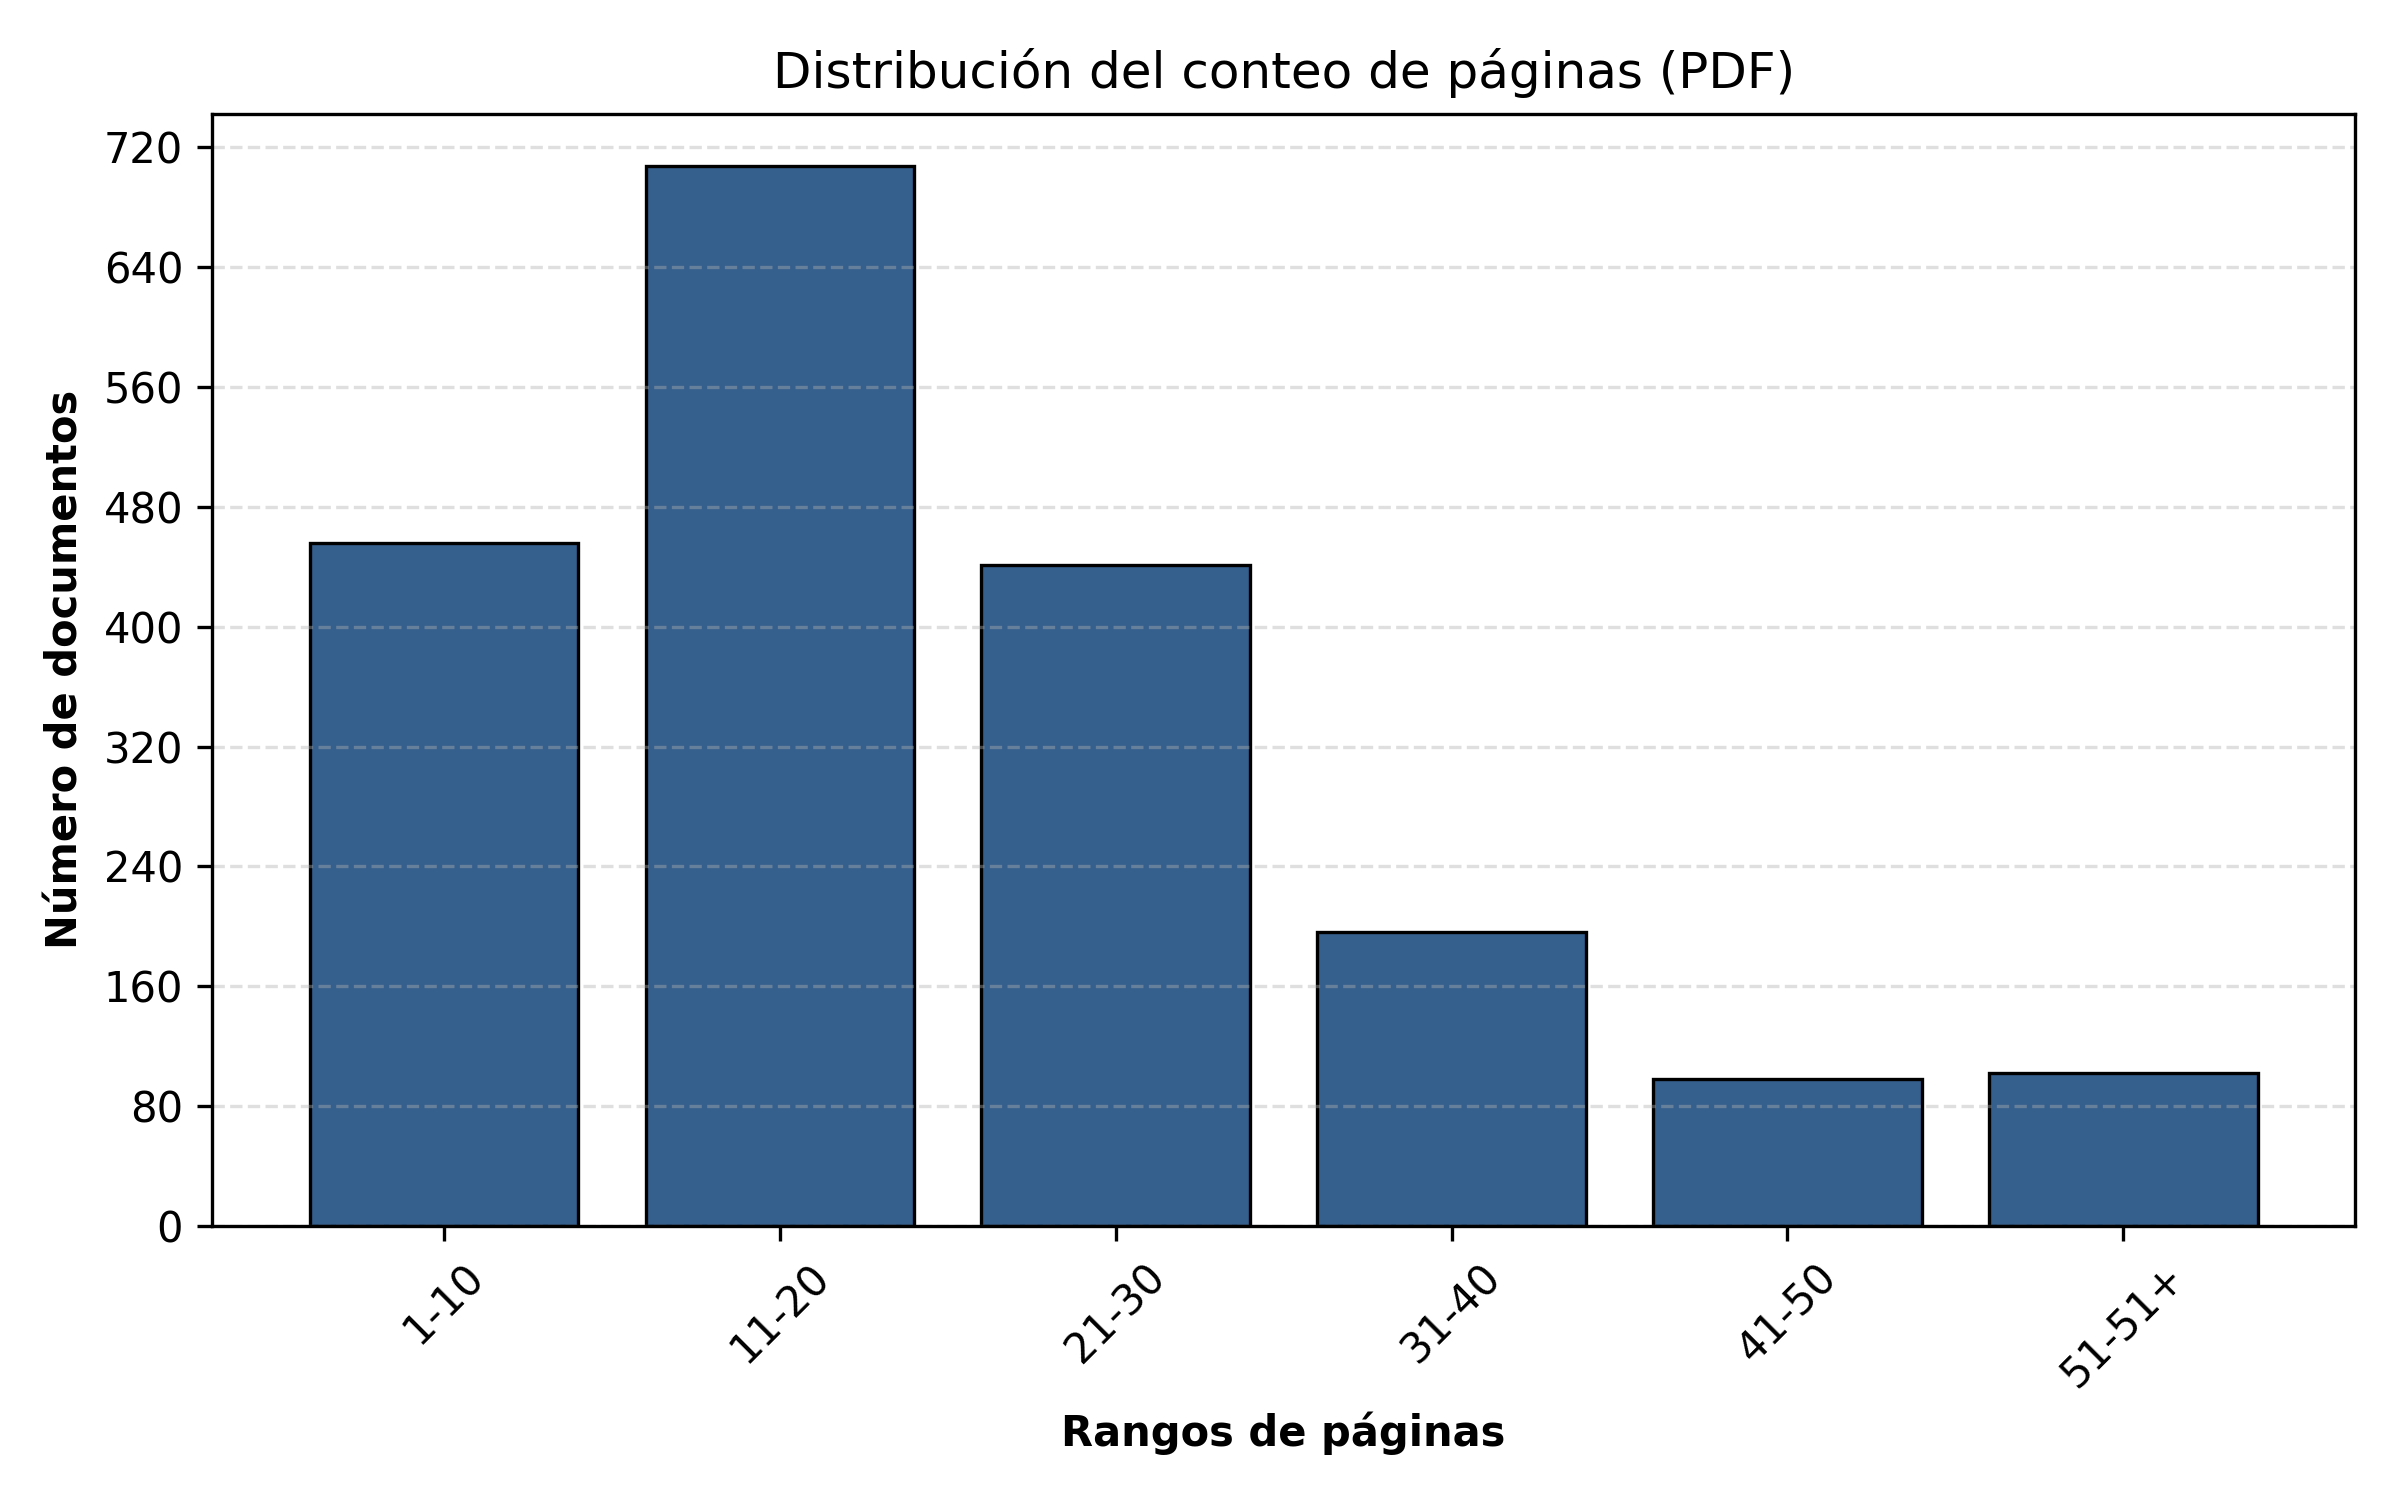
\includegraphics[width=0.8\textwidth]{page_distribution.png}
    \caption{Distribución de documentos según su extensión.}
    \label{fig:page_distribution}
\end{figure}

Por otra parte, la Figura~\ref{fig:wordcloud} presenta una representación visual de los términos más relevantes del corpus, 
donde el tamaño de cada palabra está ponderado por su importancia relativa calculada mediante la métrica TF-IDF.

\begin{figure}[ht]
    \centering
    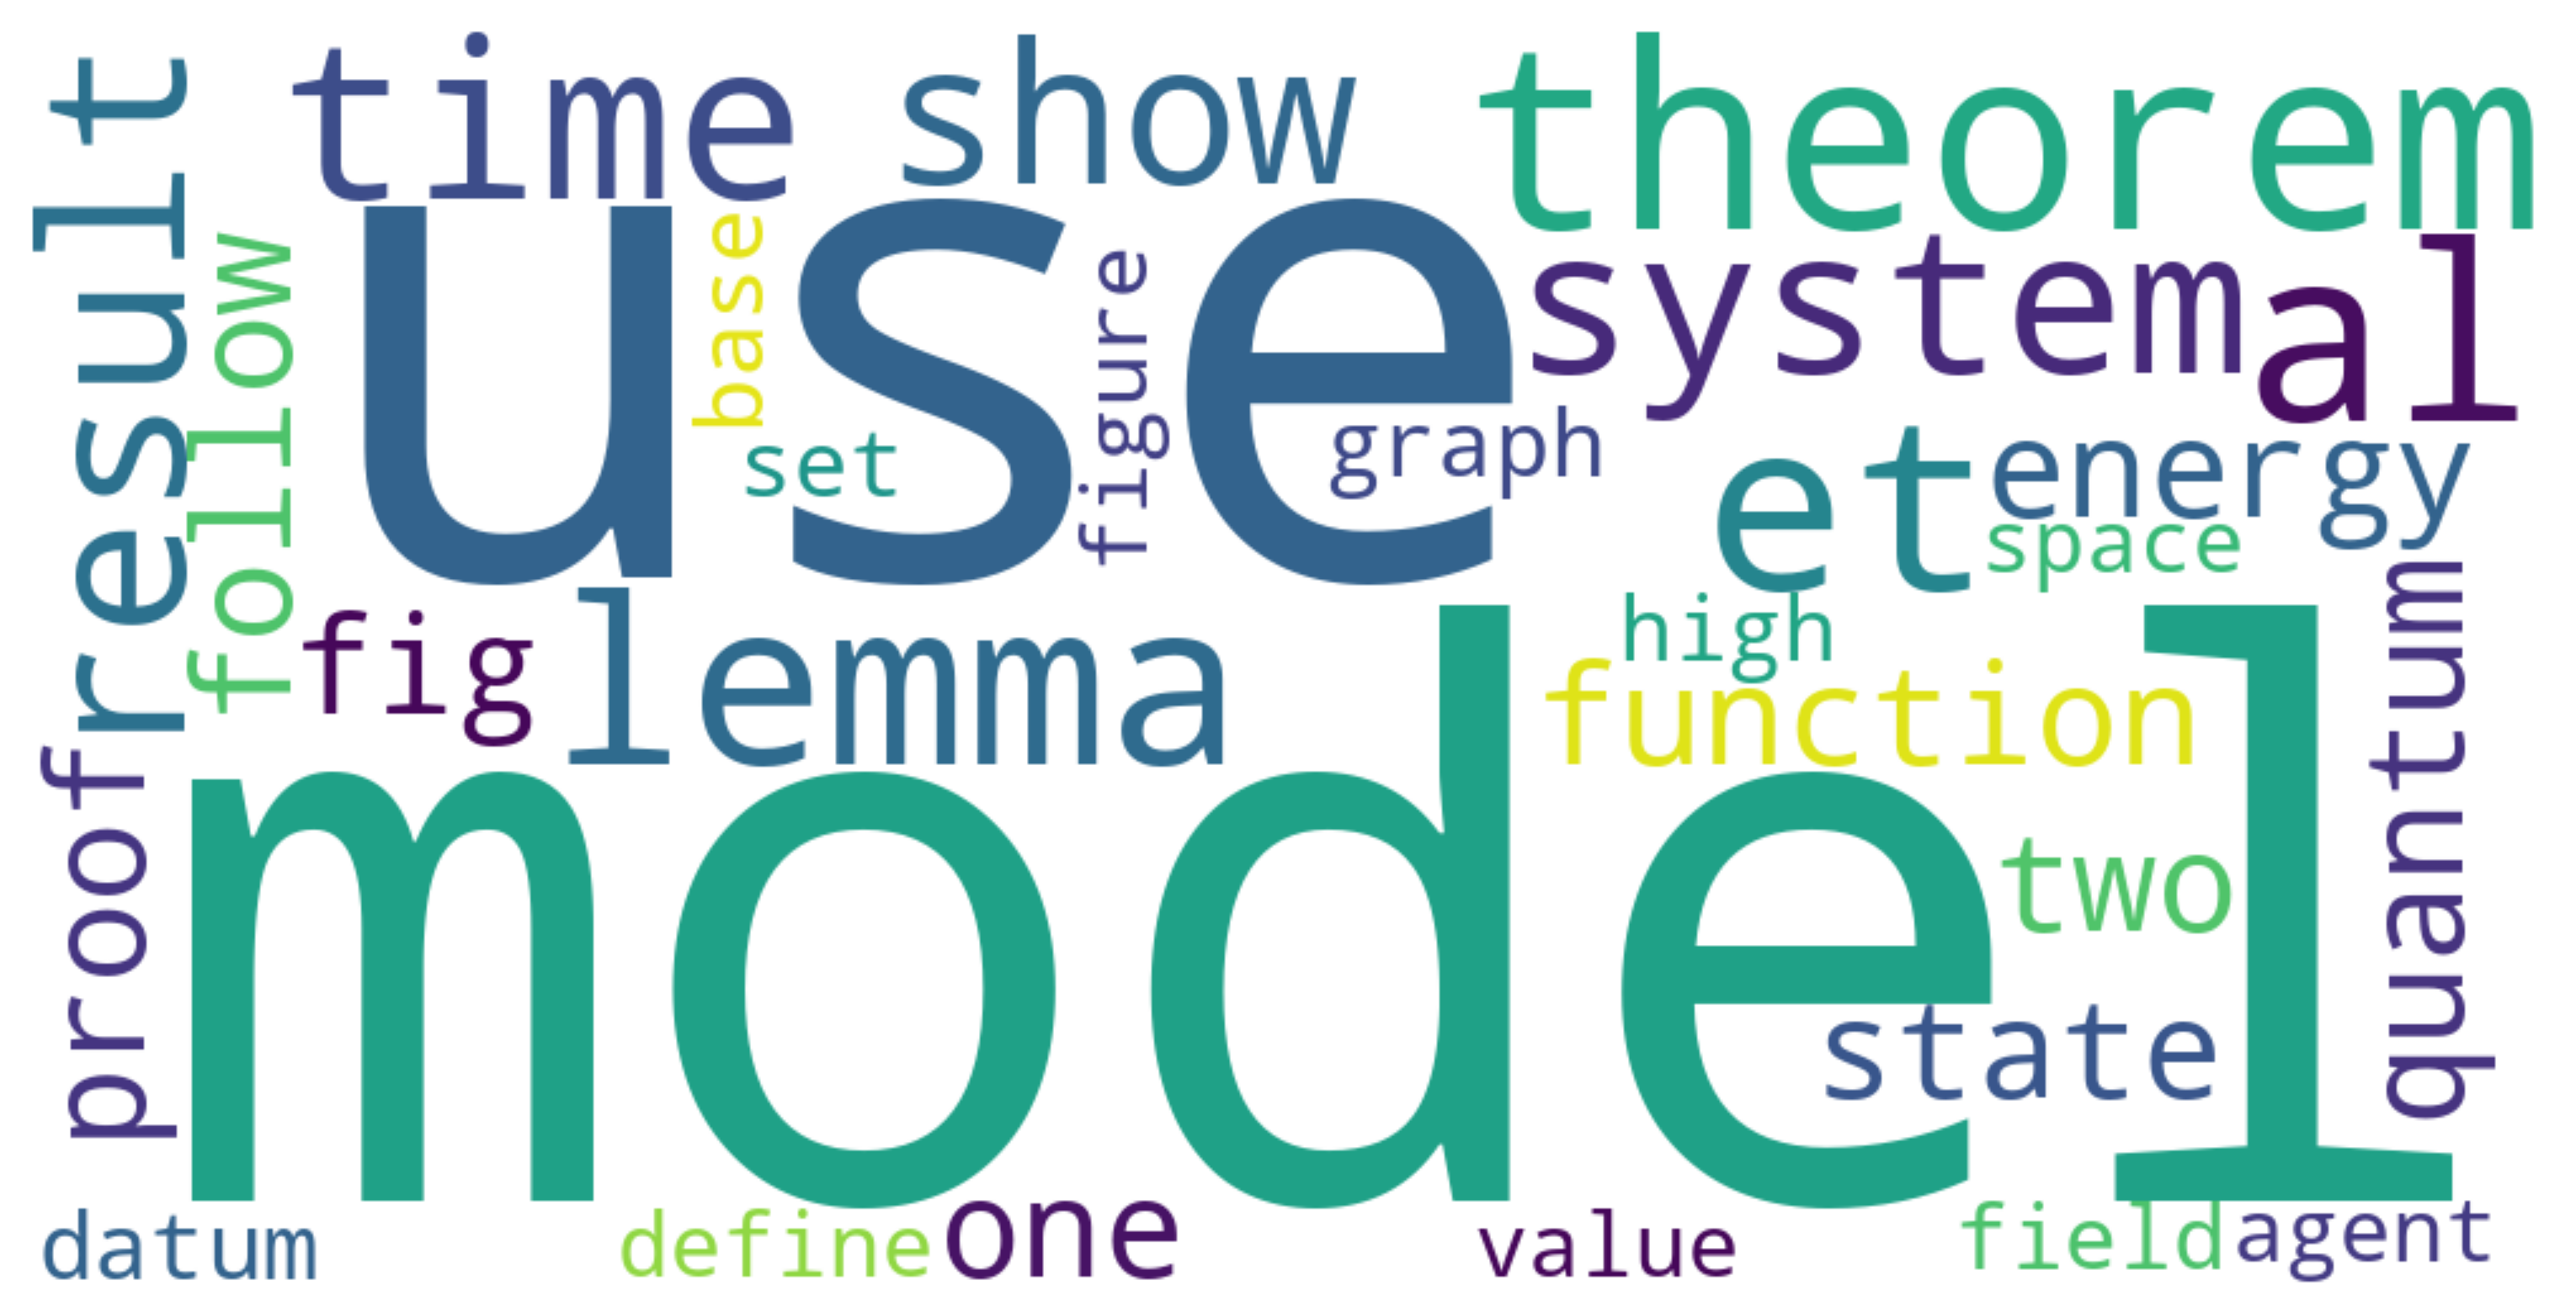
\includegraphics[width=0.8\textwidth]{wordcloud.png}
    \caption{Nube de palabras basada en puntuaciones TF-IDF.}
    \label{fig:wordcloud}
\end{figure}

En conjunto, estas estadísticas evidencian que el corpus presenta una escala y 
complejidad adecuadas para evaluar sistemas de recuperación de información en el dominio científico, 
tanto desde una perspectiva léxica como semántica.

%--------------------------------------------------
\section{Preprocesamiento del Texto}

El procesamiento de documentos científicos en formato PDF requiere una fase de normalización lingüística 
que permita transformar el texto bruto en una representación adecuada para su posterior indexación y recuperación. 
Dada la naturaleza de este dominio, donde abundan estructuras complejas, referencias bibliográficas y variabilidad terminológica, 
resulta necesario reducir el ruido y homogenizar el contenido textual. 
Esta etapa garantiza que tanto los modelos léxicos como los semánticos operen sobre datos consistentes, 
mejorando la calidad de las representaciones y, en consecuencia, la efectividad del sistema de recuperación.

El preprocesamiento se estructura como una secuencia de etapas claramente definidas:

\begin{itemize}
    \item Conversión del texto a codificación UTF-8 para eliminar caracteres inválidos.
    \item Normalización a minúsculas.
    \item Eliminación de citas mediante expresiones regulares.
    \item Tokenización del texto utilizando \textit{spaCy}, extrayendo lemas alfabéticos.
    \item Eliminación de \textit{stop words} empleando recursos de \textit{NLTK}.
    \item Aplicación de \textit{stemming} mediante el algoritmo \textit{Snowball}.
    \item Segmentación de los tokens en fragmentos (\textit{chunks}) de tamaño fijo con solapamiento.
\end{itemize}

%--------------------------------------------------
\section{Modelo de Recuperación}

El sistema implementa un enfoque de recuperación orientado al dominio científico 
que busca equilibrar precisión terminológica y comprensión semántica. 
Para ello, se integran estrategias complementarias que permiten recuperar documentos relevantes 
tanto por coincidencia exacta de términos como por similitud conceptual, 
mitigando las limitaciones inherentes a cada enfoque cuando se emplean de forma aislada.

\subsection{Recuperación Léxica (BM25F)}

La recuperación léxica se basa en la coincidencia de términos entre la consulta y los documentos, 
utilizando el modelo BM25F como función de ranking. 
Este enfoque resulta especialmente efectivo para capturar precisión terminológica y 
relevancia basada en la frecuencia y distribución de palabras clave dentro de los documentos. 
Sin embargo, su principal limitación radica en que no modela relaciones semánticas, 
por lo que puede fallar ante variaciones lingüísticas o consultas conceptuales.

\subsubsection{Modelo BM25F}

BM25F es una extensión del modelo probabilístico de recuperación BM25 \cite{bm25} propuesta en \cite{bm25f}, 
basado en el \textit{Probabilistic Relevance Framework}. 
Este enfoque estima la probabilidad de que un documento sea relevante dado una consulta, 
modelando la relevancia en función de la ocurrencia de términos. 
En su forma general, la puntuación de un documento $D$ respecto a una consulta $Q$ se define como:

\[
\text{score}(D, Q) = \sum_{t \in Q} IDF(t) \cdot \frac{f(t, D) \cdot (k_1 + 1)}{f(t, D) + k_1 \cdot \left(1 - b + b \cdot \frac{|D|}{avgdl} \right)}
\]

donde $f(t, D)$ es la frecuencia del término $t$ en el documento, $|D|$ es la longitud del documento, 
$avgdl$ es la longitud promedio de los documentos, y $k_1$, $b$ son parámetros de control. 
El término $IDF(t)$ (\textit{Inverse Document Frequency}) mide la importancia global del término:

\[
IDF(t) = \log \frac{N - df(t) + 0.5}{df(t) + 0.5}
\]

donde $N$ es el número total de documentos y $df(t)$ el número de documentos que contienen el término.

La variante BM25F introduce el concepto de \textit{fields} (campos), 
permitiendo ponderar distintas partes estructurales del documento, como título, resumen o contenido. 
En este caso, la frecuencia efectiva del término se calcula como una combinación ponderada por campo:

\[
f(t, D) = \sum_{c \in C} w_c \cdot \frac{f(t, D_c)}{1 - b_c + b_c \cdot \frac{|D_c|}{avgdl_c}}
\]

donde $c$ representa cada campo (por ejemplo, \textit{title}, \textit{abstract}, \textit{content}), 
$w_c$ es el peso asignado al campo, y $b_c$ controla la normalización por longitud dentro de cada campo. 
Esta formulación permite dar mayor importancia a campos más informativos, como el título o el resumen, 
lo cual es especialmente relevante en documentos científicos. 
En la implementación, se utilizan pesos diferenciados por campo y parámetros ajustados ($k_1=1.7$, $b=0.65$), 
junto con un filtrado relativo sobre los resultados para conservar únicamente aquellos cuya puntuación sea cercana 
a la máxima obtenida.

\subsection{Recuperación Semántica (Embeddings)}

La recuperación semántica se basa en el uso de representaciones vectoriales densas 
generadas mediante modelos de redes neuronales profundas. 
En particular, se emplea un modelo de \textit{Sentence Transformers} \cite{sentence_transformers}, 
específicamente \textit{multi-qa-mpnet-base-dot-v1}, basado en arquitecturas tipo Transformer, 
que permite codificar tanto consultas como fragmentos de texto (\textit{chunks}) en vectores de dimensión fija 
dentro de un espacio semántico continuo. 
En este espacio, la proximidad entre vectores refleja similitud conceptual, 
lo que permite recuperar información relevante incluso en ausencia de coincidencias léxicas explícitas.
No obstante, este enfoque puede perder precisión en la recuperación de términos específicos o altamente técnicos.

\subsubsection{Dense Embeddings}

Para la indexación, cada \textit{chunk} de texto es transformado en un embedding y 
almacenado en un índice vectorial utilizando FAISS \cite{faiss}. 
Antes de su inserción, los vectores son normalizados, 
lo que permite utilizar el producto interno como medida de similitud equivalente al coseno. 
Durante la recuperación, la consulta es igualmente codificada en un vector, 
y el sistema realiza una búsqueda de los vectores más cercanos en el índice, 
retornando aquellos cuya similitud supera un umbral definido. 
Este mecanismo permite identificar fragmentos relevantes 
mediante comparaciones vectoriales eficientes en espacios de alta dimensión.

\subsubsection{Modelo de Similitud Vectorial}

El modelo de recuperación semántica se basa en la comparación entre vectores normalizados en un espacio euclidiano. 
Dado un embedding de consulta $q \in \mathbb{R}^d$ y un embedding de documento $d_i \in \mathbb{R}^d$, 
ambos normalizados, la similitud se calcula mediante el producto interno:

\[
\text{sim}(q, d_i) = q \cdot d_i = \sum_{j=1}^{d} q_j \cdot d_{i,j}
\]

Dado que los vectores están normalizados a norma unitaria, esta operación es equivalente a la similitud del coseno:

\[
\text{sim}(q, d_i) = \cos(\theta) = \frac{q \cdot d_i}{\|q\| \|d_i\|}
\]

El proceso de recuperación consiste en resolver el problema de \textit{nearest neighbor search}, 
es decir, encontrar los $k$ vectores $d_i$ que maximizan $\text{sim}(q, d_i)$. 
Para ello, se utiliza un índice FAISS con métrica de producto interno, 
optimizado para búsquedas eficientes en grandes colecciones de vectores. 
Finalmente, se aplica un umbral de similitud para filtrar resultados poco relevantes y 
se ordenan los candidatos en función de su puntuación.

\subsection{Recuperación Híbrida}

La recuperación híbrida combina los enfoques léxico y semántico para aprovechar sus fortalezas complementarias, 
lo cual resulta especialmente necesario en el dominio científico. 
El sistema genera dos listas de resultados independientes, una por cada modelo, 
que posteriormente se integran mediante un mecanismo de fusión de rankings basado en RRF. 
Esta estrategia permite obtener un orden final más robusto y consistente, mejorando la calidad global de la recuperación.

%--------------------------------------------------
\section{Persistencia}

El sistema emplea múltiples mecanismos de persistencia especializados según el tipo de dato. 
Los embeddings densos se almacenan en un índice FAISS, donde se guardan como vectores normalizados 
para permitir búsquedas eficientes por similitud semántica. 
En paralelo, Whoosh gestiona el índice léxico, almacenando los documentos estructurados en campos 
(título, resumen, contenido) para su recuperación mediante BM25F.

Adicionalmente, los fragmentos de texto (\textit{chunks}) se almacenan en una base de datos SQLite, 
lo que permite su recuperación posterior durante el proceso de RAG. 
Finalmente, los metadatos asociados a los embeddings (como identificadores de chunks y documentos) 
se serializan mediante \textit{pickle}, facilitando la correspondencia entre los vectores recuperados y su contenido original.

%--------------------------------------------------
\section{Ranking y Posicionamiento}

El módulo de ranking y posicionamiento recibe como entrada dos conjuntos de resultados independientes 
provenientes de los dos subsistemas de recuperación implementados: 
el modelo léxico basado en BM25F y el modelo semántico basado en embeddings densos. 
Es importante destacar que ninguno de estos recuperadores devuelve el conjunto completo de documentos indexados, 
sino únicamente subconjuntos filtrados de candidatos potencialmente relevantes, 
los cuales serán posteriormente fusionados para construir el ranking final.

En el caso del recuperador léxico (BM25F), el sistema obtiene una puntuación asociada a cada documento mediante el motor Whoosh. 
A partir del mayor score obtenido en la consulta (\textit{best score}), 
se define un umbral dinámico de relevancia como $score\_threshold = best \cdot 0.9$. 
Únicamente se conservan aquellos documentos cuyo score es mayor o igual a este umbral, 
lo que permite reducir la lista inicial a los resultados más relevantes según coincidencia terminológica.

Por su parte, el recuperador semántico basado en embeddings calcula la similitud entre la consulta y los \textit{chunks} 
mediante un modelo vectorial, produciendo un score de similitud en el espacio latente. 
En este caso, se aplica un umbral fijo de filtrado definido como $chunk\_similarity\_threshold = 0.5$, 
conservando únicamente aquellos fragmentos cuya similitud supera dicho valor. 
De esta manera, ambos recuperadores entregan al módulo de ranking conjuntos reducidos y filtrados de candidatos relevantes, 
que posteriormente serán fusionados mediante estrategias de agregación de rankings.

\subsection{Ranking algorítmico}

El sistema emplea \textit{Reciprocal Rank Fusion} (RRF) como mecanismo de fusión para integrar los resultados 
provenientes de los recuperadores léxico y semántico. 
Este método permite combinar múltiples rankings sin requerir que ambos contengan exactamente los mismos documentos, 
privilegiando aquellos que aparecen en posiciones altas en varias listas. 
Como resultado, se obtiene una ordenación final más robusta, al reducir la dependencia de un único modelo de recuperación.

El uso de RRF resulta especialmente adecuado en un sistema híbrido, 
ya que permite integrar evidencia léxica y semántica de manera efectiva. 
Esta estrategia mitiga la fragilidad de rankings individuales y mejora la estabilidad del orden final, 
favoreciendo documentos que son consistentemente relevantes bajo distintos criterios.

\subsubsection{Reciprocal Rank Fusion (RRF)}

RRF \cite{rrf} combina múltiples rankings asignando a cada documento una puntuación basada en su posición en cada lista. 
Formalmente, dado un conjunto de rankings $R = \{r_1, r_2, ..., r_m\}$, la puntuación de un documento $d$ se define como:

\[
\text{RRF}(d) = \sum_{r \in R} \frac{1}{k + \text{rank}_r(d)}
\]

donde $\text{rank}_r(d)$ es la posición de $d$ en el ranking $r$, y 
$k$ es una constante positiva (típicamente ajustada a $60$) que atenúa la contribución de posiciones bajas. 
Este esquema favorece documentos bien posicionados en múltiples rankings, 
sin penalizar excesivamente aquellos que no aparecen en todas las listas.

\subsection{Posicionamiento visual}

Los resultados recuperados se presentan al usuario en orden descendente de relevancia, 
priorizando aquellos documentos con mayor puntuación final.
Adicionalmente, el sistema permite no solo la descarga de los documentos PDF recuperados, 
sino también una previsualización (\textit{preview}) de su contenido, lo que facilita una inspección rápida 
sin necesidad de abandonar el entorno de consulta. 
Esta estructura mejora la exploración interactiva del corpus y permite al usuario evaluar la pertinencia 
de los resultados de forma más eficiente.

%--------------------------------------------------
\section{Expansión de Consultas y Retroalimentación}

\subsection{Expansión de Consultas}

El sistema implementa un mecanismo de expansión de consultas basado en retroalimentación implícita 
de la primera fase de recuperación (formalmente desarrollado en \cite{pseudo_relevance}), cuyo comportamiento conceptual se ilustra en la Figura~\ref{fig:query_expansion}. 
Inicialmente, se realiza una búsqueda con la consulta original, a partir de la cual se obtienen 
\textit{chunks} candidatos que presentan coincidencia o alta similitud semántica. 
Posteriormente, el contenido de estos fragmentos se combina con la consulta inicial para construir una representación enriquecida, 
la cual es nuevamente vectorizada mediante el modelo de embeddings, 
generando una nueva representación más informada del contexto de búsqueda.

Este proceso permite ejecutar una segunda fase de recuperación más precisa, ya que la consulta expandida incorpora términos y 
conceptos presentes en los documentos inicialmente recuperados. 
En el dominio de la literatura científica, esta estrategia mejora significativamente la calidad de la búsqueda 
al desambiguar consultas cortas, incorporar vocabulario relevante del contexto y 
aumentar el \textit{recall} sin degradar de forma sustancial la precisión del sistema.

\begin{figure}[ht]
    \centering
    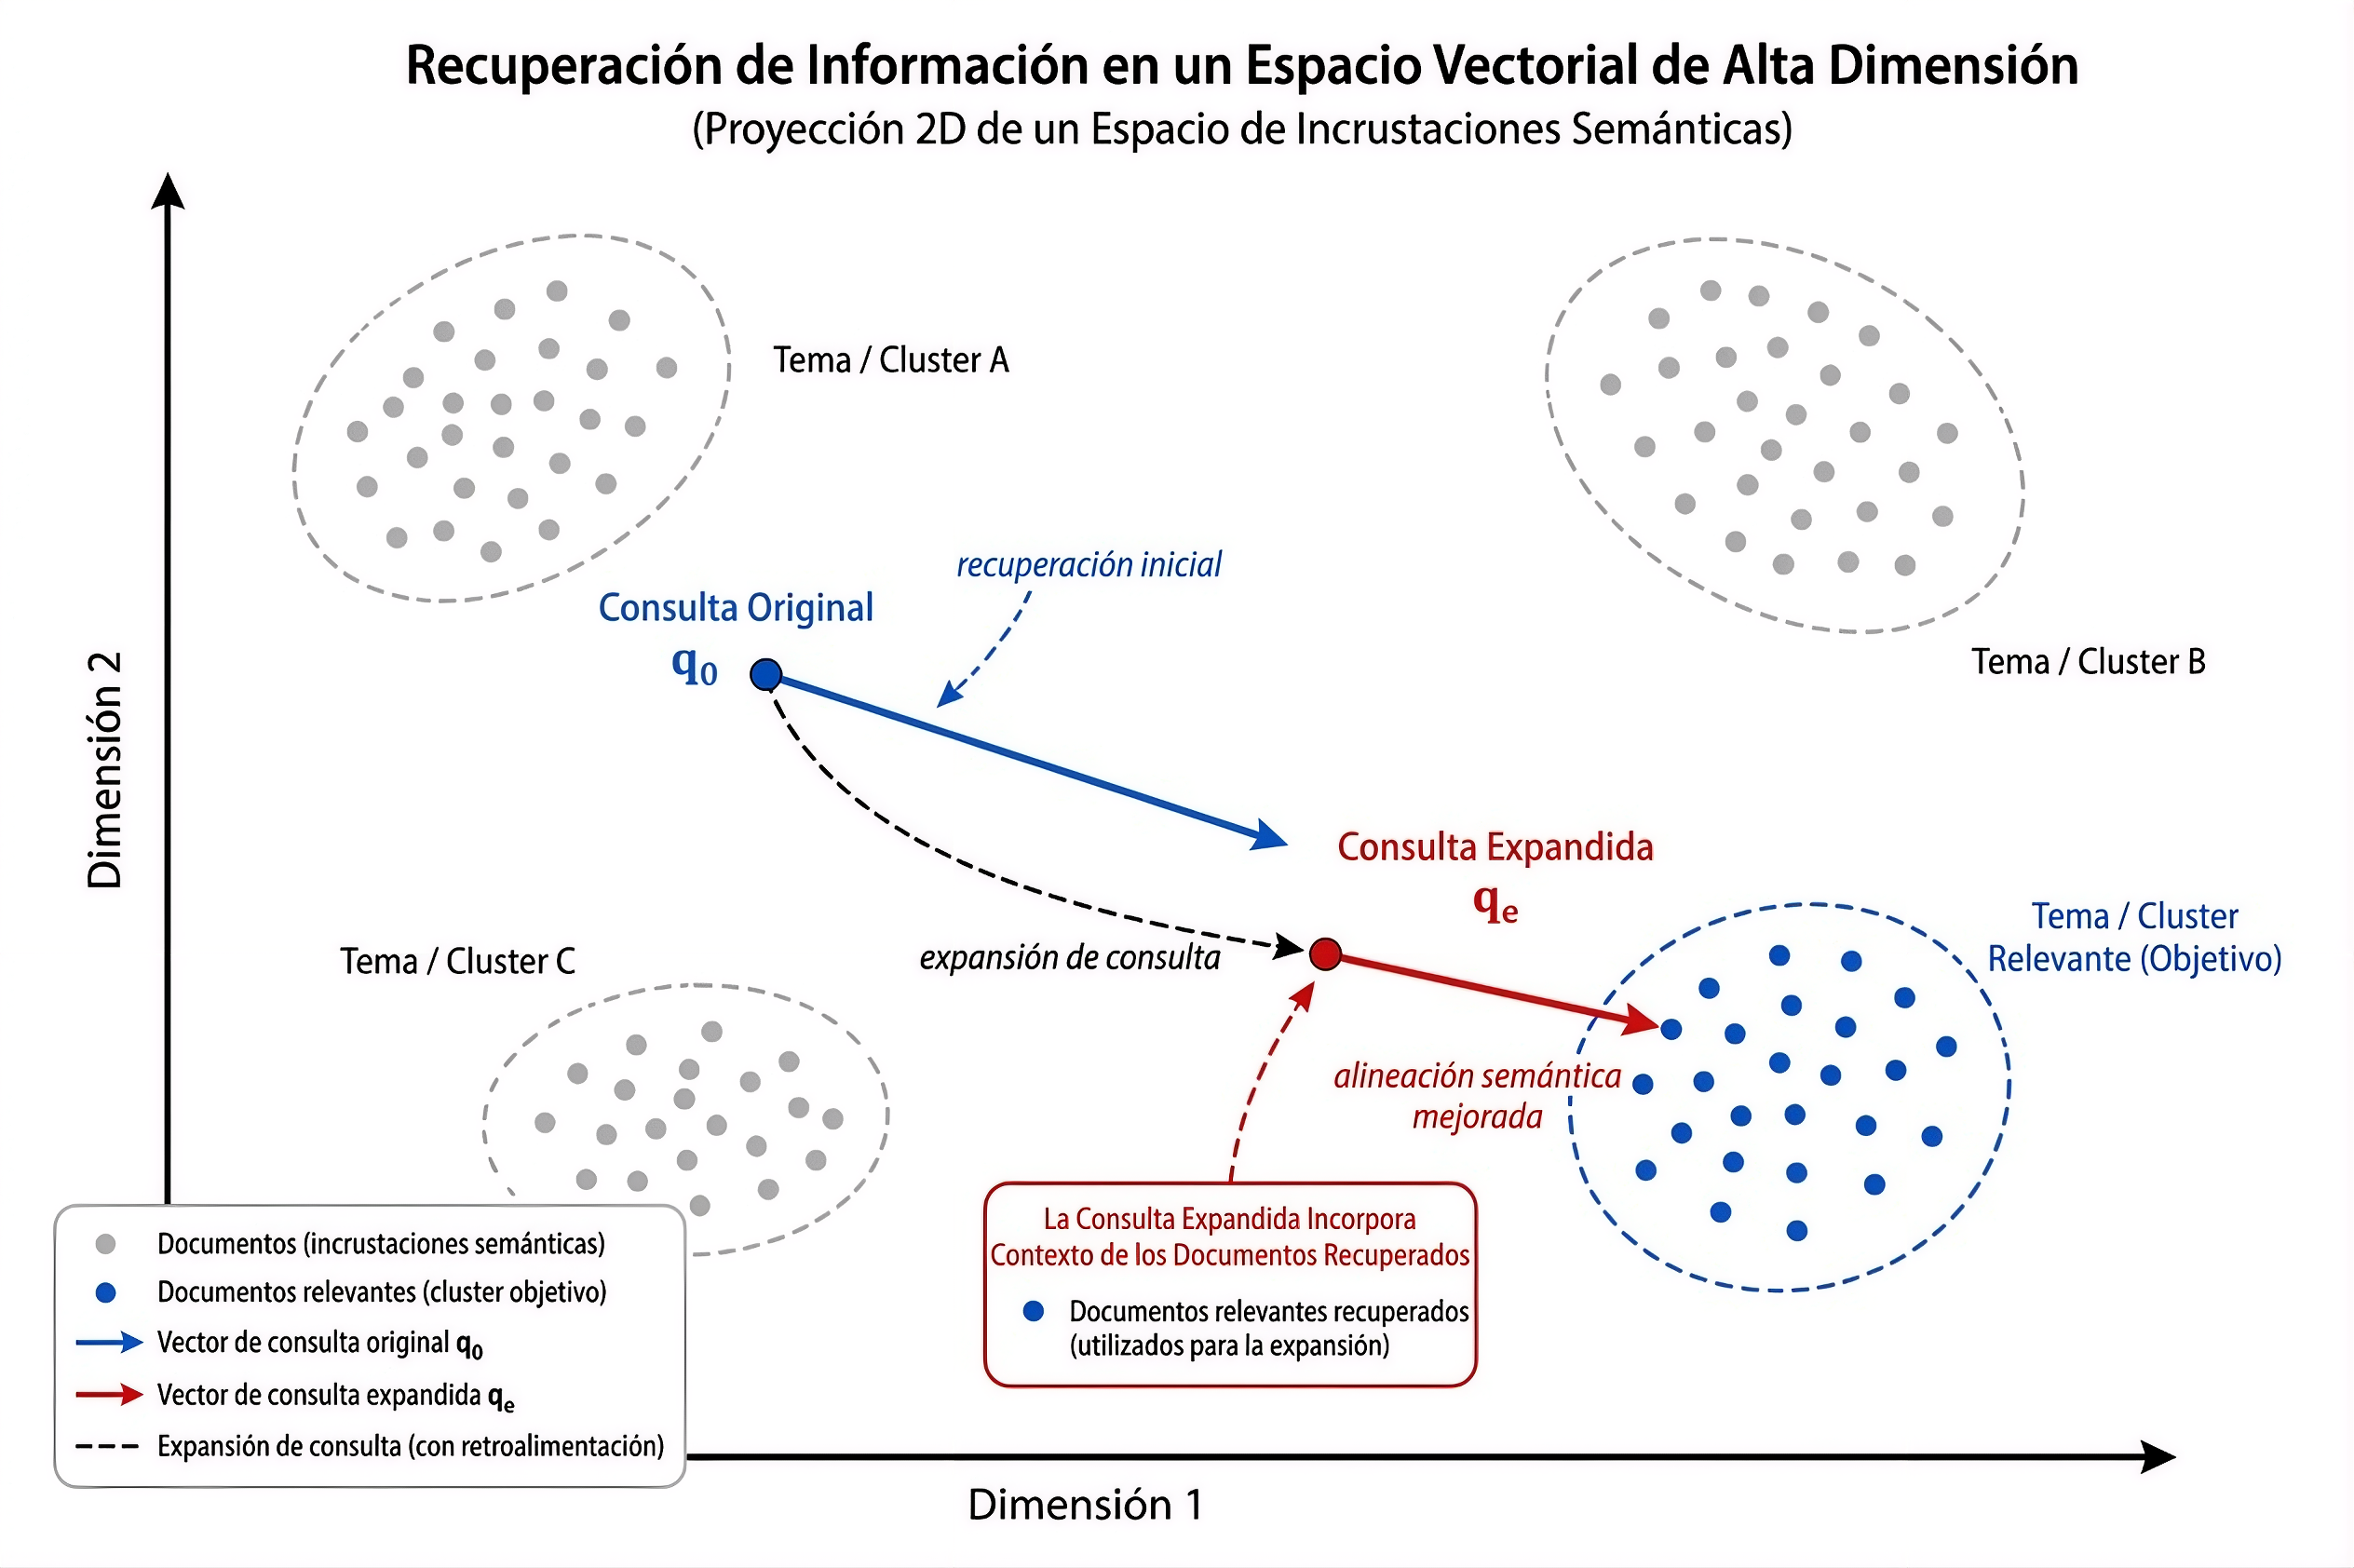
\includegraphics[width=0.85\textwidth]{query_expansion.png}
    \caption{Efecto de la expansión de consultas en el espacio vectorial semántico. 
    La consulta original se reubica mediante la incorporación de contexto recuperado, 
    mejorando su alineación con documentos relevantes.}
    \label{fig:query_expansion}
\end{figure}

\subsection{Módulo de Feedback (Trabajo Futuro)}

%--------------------------------------------------
\section{Módulo RAG}

El sistema integra un esquema de \textit{Retrieval-Augmented Generation} (RAG \cite{rag}) con el objetivo de no limitarse únicamente a 
la recuperación de documentos, sino también generar respuestas enriquecidas a partir de la evidencia obtenida. 
En este enfoque, la consulta del usuario es primero procesada y expandida para mejorar su representatividad semántica. 
Posteriormente, se construye un contexto a partir de los \textit{chunks} relevantes recuperados por los módulos de búsqueda, 
los cuales son agregados en una representación textual estructurada.

Este contexto es posteriormente incorporado a un \textit{prompt} 
que se envía a un modelo generativo alojado en Cloudflare \cite{cloudflare}, 
\texttt{@cf/meta/llama-3.1-8b-instruct}. 
El modelo produce una respuesta condicionada por la evidencia recuperada, 
diferenciando explícitamente entre información derivada del contexto y conocimiento general del modelo cuando sea necesario. 
De este modo, la respuesta no se genera únicamente a partir de memoria paramétrica, 
sino que está fundamentada en documentos recuperados del corpus.

Este enfoque resulta particularmente útil en el dominio de la literatura científica, 
ya que permite responder preguntas complejas, sintetizar información proveniente de múltiples fuentes y 
facilitar la exploración del corpus mediante respuestas explicativas. 
Es importante destacar que el módulo RAG no sustituye el proceso de recuperación, sino que lo complementa: 
primero se obtiene evidencia relevante y posteriormente se genera una respuesta asistida por el modelo de lenguaje, 
lo que mejora la expresividad y utilidad del sistema sin comprometer la trazabilidad de la información.

%--------------------------------------------------
\section{Módulo de Búsqueda Web}

El sistema incorpora un módulo de búsqueda web como mecanismo de ampliación dinámica del corpus, 
el cual se activa automáticamente cuando los resultados recuperados no alcanzan un nivel mínimo de relevancia o 
cantidad según un umbral definido sobre el ranking obtenido. 
Este comportamiento permite detectar situaciones en las que la base local no contiene suficiente información 
para responder adecuadamente a la consulta del usuario.

Cuando se activa, el módulo utiliza la API de arXiv para realizar una búsqueda externa basada en la consulta original del usuario. 
A partir de los resultados obtenidos, se descargan nuevos documentos en formato PDF, 
los cuales son incorporados al sistema para su posterior procesamiento e indexación. 
Este proceso respeta estrictamente las políticas definidas en el archivo \texttt{robots.txt}, 
incluyendo las rutas permitidas (\textit{allowed URLs}) y las restricciones de acceso temporal (\textit{crawl\_delay}), 
garantizando un comportamiento conforme a las normas del servidor.

Este enfoque es especialmente relevante en el dominio de la investigación científica, 
donde la literatura evoluciona continuamente, el corpus local puede volverse rápidamente incompleto y 
no siempre es posible garantizar cobertura total de los temas consultados. 
En este sentido, la búsqueda web actúa como un mecanismo de actualización y expansión del sistema, 
asegurando mayor cobertura y pertinencia en las respuestas generadas.

%--------------------------------------------------
\section{Sistema de Recomendación}

El sistema incorpora un módulo de recomendación basado en el historial de interacciones del usuario con la interfaz 
(tomando como referencia \cite{recsys}), 
el cual registra información sobre consultas realizadas y documentos consultados. 
Este historial permite construir un perfil implícito de usuario, 
donde se modelan sus intereses a partir de las temáticas recurrentes en sus búsquedas y 
de los contenidos con los que interactúa con mayor frecuencia.

A partir de este perfil, el sistema genera recomendaciones de documentos relacionados con las consultas previas y 
con los resultados recuperados recientemente, priorizando aquellos contenidos que presentan similitud temática con 
el comportamiento histórico del usuario. 
Estas recomendaciones se integran como una capa adicional sobre el sistema de recuperación, 
complementando los resultados principales sin interferir con el proceso de ranking.

En el dominio de la investigación científica, este enfoque resulta especialmente útil debido a 
la naturaleza iterativa de las búsquedas, donde los usuarios suelen explorar temas consistentes a lo largo del tiempo y 
reformular consultas relacionadas. 
En este contexto, la recomendación actúa como un mecanismo de personalización que mejora la exploración del corpus, 
sin sustituir el núcleo del sistema de recuperación de información.

%--------------------------------------------------
\section{Interfaz Visual}

\subsection{Descripción General}

La interfaz visual del sistema está implementada utilizando Streamlit \cite{streamlit}, 
lo que permite construir una aplicación web interactiva con una arquitectura simple y modular. 
La interfaz se organiza en tres páginas principales: 
una dedicada a recomendaciones, otra enfocada en la recuperación de información, 
y una tercera orientada a la interacción tipo chat con el módulo RAG. 
En la parte superior de todas las páginas se dispone de una barra de navegación con tres botones que 
permiten el cambio entre vistas de forma consistente.

La primera página muestra recomendaciones personalizadas basadas en el historial de interacción del usuario, 
facilitando el acceso a documentos potencialmente relevantes. 
La segunda página constituye el núcleo del sistema de recuperación, 
donde el usuario introduce su consulta en una barra de búsqueda y recibe como salida una lista de documentos recuperados, 
con opciones de previsualización y descarga de los PDFs. 
La tercera página implementa una interfaz tipo chat que permite interactuar con el sistema generativo, 
donde las respuestas se construyen a partir del módulo RAG, 
ofreciendo una experiencia conversacional para la exploración del contenido, 
este tipo de interacción es familiar al usuario aunque el módulo realmente no funcione como un chat.

\subsection{Decisiones de Diseño}

El diseño de la interfaz prioriza una estructura clara y jerárquica que facilite la navegación y 
la comprensión de la información. 
La organización en tres vistas separadas permite desacoplar las funcionalidades principales del sistema: 
recomendación, recuperación y generación. 
Esta separación contribuye a reducir la carga cognitiva del usuario y mejora la claridad en el flujo de interacción.

Se adopta un estilo visual moderno y minimalista basado en una paleta de colores blanco, negro y gris, 
con acentos en color morado para elementos interactivos como botones, efectos \textit{hover} y acciones destacadas. 
La disposición de los elementos prioriza la visibilidad de la barra de búsqueda y los resultados más relevantes, 
asegurando una jerarquía visual coherente donde la consulta, los resultados y 
la respuesta generada se presentan de forma claramente diferenciada. 
Este diseño busca optimizar la legibilidad, facilitar la comparación de resultados y 
mejorar la experiencia de exploración del sistema.

%--------------------------------------------------
\section{Documentación Técnica Completa del Sistema}

Desde una perspectiva de ingeniería de software, el sistema se organiza como una arquitectura modular por capas, 
donde cada componente cumple una función específica dentro del flujo global de recuperación de información. 
El sistema completo está coordinado por un \textit{backend controller}, 
el cual actúa como punto central de decisión y orquestación entre los distintos módulos, 
mientras que el \textit{frontend} basado en Streamlit se encarga exclusivamente de la interacción con el usuario.

El flujo principal de ejecución se inicia en la interfaz, donde el usuario introduce una consulta o interactúa con el sistema. 
Esta entrada es enviada al \textit{backend controller}, el cual determina el tipo de operación a realizar: 
búsqueda, recomendación o generación RAG. 
Independientemente del caso, el sistema transforma la entrada en una consulta procesada que puede ser expandida, 
y posteriormente invoca el módulo de ranking. 
Este módulo delega la recuperación a los sistemas BM25F y embeddings densos, cuyos resultados son fusionados mediante RRF. 
En caso de que la evidencia recuperada sea insuficiente según un umbral definido, 
se activa automáticamente el módulo de búsqueda web, el cual descarga nuevos documentos, 
los indexa nuevamente mediante los módulos de indexación léxica y semántica, y reintegra los resultados al proceso de ranking. 
Finalmente, los resultados son devueltos al frontend para su visualización.

Por otro lado, existen procesos independientes de construcción del corpus basados en \textit{crawling} y \textit{scraping}, 
los cuales operan fuera del flujo interactivo de la interfaz. 
Estos módulos permiten la recolección y descarga de documentos PDF desde arXiv, generando la base documental inicial del sistema. 
Una vez obtenidos los documentos, el módulo de indexación puede ser ejecutado para construir y actualizar 
tanto el índice BM25F como el índice vectorial denso, asegurando la disponibilidad de los datos para los procesos de recuperación.

\subsection{Arquitectura por Capas}

\subsubsection{Capa de Adquisición}
Esta capa incluye los módulos de \textit{crawling}, \textit{scraping} y la integración con la API de arXiv, 
responsables de la recolección de documentos desde la web y la construcción inicial del corpus.

\subsubsection{Capa de Procesamiento}
Encargada del preprocesamiento del texto, incluye normalización, limpieza, tokenización, eliminación de ruido, 
generación de hashes y segmentación en \textit{chunks}.

\subsubsection{Capa de Indexación}
Gestiona la construcción y mantenimiento de los índices léxicos (BM25F) y vectoriales (embeddings), 
así como la persistencia de \textit{chunks} y representaciones intermedias.

\subsubsection{Capa de Recuperación}
Incluye los recuperadores BM25F y denso, el módulo de expansión de consultas y el mecanismo de fusión de resultados mediante RRF.

\subsubsection{Capa de Generación y Presentación}
Integra el módulo RAG y la interfaz Streamlit, encargada de la visualización de resultados, respuestas generadas y 
navegación del usuario.

\subsubsection{Capa de Personalización}
Basada en el historial de interacción del usuario, alimenta el sistema de recomendación y 
contribuye a la adaptación de los resultados a los intereses del usuario.

%--------------------------------------------------
\section{Manual de Usuario}

Este sistema está diseñado para ser ejecutado como una aplicación web local, 
sin requerir conocimiento del código fuente. 
A continuación se describen los pasos necesarios para su instalación, ejecución y uso básico.

\subsection{Instalación y Ejecución}

Para comenzar, se debe clonar el repositorio del proyecto:

\begin{verbatim}
git clone https://github.com/John31415/beagle-ir.git
cd beagle-ir
\end{verbatim}

Posteriormente, se crea y activa un entorno virtual de Python:

\begin{verbatim}
# Linux / macOS
python3 -m venv venv
source venv/bin/activate

# Windows
python -m venv venv
venv\Scripts\activate
\end{verbatim}

Luego se instalan las dependencias del sistema:

\begin{verbatim}
pip install -r requirements.txt
\end{verbatim}

Finalmente, la interfaz se ejecuta mediante Streamlit:

\begin{verbatim}
streamlit run frontend/interface.py
\end{verbatim}

Una vez ejecutado, el sistema estará disponible en el navegador en la dirección \texttt{http://localhost:8501}.

\subsection{Construcción y Actualización del Corpus}

La construcción del corpus se realiza mediante el módulo de adquisición de datos. 
Para activarlo, es necesario descomentar la función \texttt{create\_corpus()} en el archivo \texttt{arxiv\_corpus.py} y ejecutar:

\begin{verbatim}
python3 -m data_ingestion.arxiv_corpus
\end{verbatim}

Este proceso descarga documentos desde arXiv respetando restricciones como \textit{crawl\_delay}, 
límites de descarga y ancho de banda, por lo que puede tardar varias horas.

Una vez descargado el corpus, los índices deben ser generados o actualizados. 
Para ello se debe descomentar la función \texttt{build\_indexes()} en \texttt{build\_indexes.py} y ejecutar:

\begin{verbatim}
python3 -m indexing.build_indexes
\end{verbatim}

Este paso construye tanto el índice léxico como el índice vectorial necesarios para la recuperación de información.

\subsection{Uso del Sistema}

El usuario interactúa con el sistema exclusivamente a través de 
tres vistas independientes accesibles desde la barra de navegación superior. 
En cada una de ellas, la interacción se reduce a acciones simples: 
navegación entre páginas, escritura en una barra de búsqueda o interacción mediante un chat, 
sin necesidad de configurar parámetros adicionales.

En la vista de recuperación de información, el usuario introduce una consulta en la barra de búsqueda. 
A partir de esta entrada, el sistema ejecuta el proceso de recuperación y presenta una lista de documentos relevantes. 
Cada resultado puede ser previsualizado o descargado en formato PDF, permitiendo una exploración directa del contenido.

En la vista de recomendaciones, el usuario no realiza acciones adicionales más allá de la navegación, 
ya que los documentos sugeridos se generan automáticamente a partir del historial de interacción. 
Finalmente, en la vista de chat RAG, el usuario escribe preguntas en un entorno conversacional. 
El sistema responde con una salida generada a partir de información recuperada del corpus, 
presentada como una respuesta textual continua, independiente del listado de documentos.

Estas tres formas de interacción son completamente independientes entre sí y responden a distintos modos de uso del sistema: 
exploración directa del corpus, consulta puntual y asistencia conversacional.

%--------------------------------------------------
\section{Discusión}

\subsection{Bondades del Sistema}

El sistema propuesto integra de forma coherente múltiples enfoques de recuperación de información, 
combinando modelos léxicos basados en BM25F con representaciones semánticas mediante embeddings densos. 
Esta hibridación permite capturar tanto coincidencias terminológicas exactas como similitud conceptual, 
lo que resulta especialmente adecuado para el dominio de la literatura científica.

Adicionalmente, el uso de un corpus real obtenido desde arXiv aporta relevancia práctica al sistema, 
mientras que la incorporación de un mecanismo de búsqueda web dinámica permite ampliar la cobertura de información 
cuando el repositorio local no es suficiente. 
La inclusión de un módulo RAG añade capacidad de síntesis generativa basada en evidencia recuperada, 
mejorando la expresividad del sistema sin perder trazabilidad.

Desde el punto de vista de ingeniería, la arquitectura modular facilita la separación de responsabilidades entre adquisición, 
procesamiento, indexación, recuperación, ranking y presentación. 
Finalmente, la interfaz visual implementada proporciona una experiencia de uso funcional y estructurada, 
permitiendo la exploración del sistema de manera intuitiva.

\subsection{Limitaciones}

A pesar de sus ventajas, el rendimiento global del sistema depende fuertemente de la calidad y cobertura del corpus construido.

La expansión de consultas, aunque útil para mejorar el recall, puede introducir ruido en escenarios donde 
la recuperación inicial es débil o poco precisa. 
Por otro lado, la generación de respuestas mediante el modelo LLM puede requerir validación adicional en contextos científicos, 
ya que existe el riesgo de incorporar inferencias no estrictamente soportadas por el contexto recuperado.

Finalmente, el procesamiento de documentos PDF puede verse afectado por ruido en la extracción de texto, 
especialmente en casos de formateo complejo o contenido mal estructurado, 
lo cual impacta directamente en la calidad de los índices construidos.

%--------------------------------------------------
\section{Trabajo Futuro}

A partir del análisis del sistema implementado, se identifican varias líneas de mejora orientadas a incrementar la robustez, 
cobertura y calidad de los resultados. 
En primer lugar, el ruido generado durante la extracción de texto desde documentos PDF constituye una 
fuente importante de degradación en la calidad del corpus. 
Como posible solución, se propone mejorar las técnicas de \textit{parsing}, 
así como refinar los procesos de limpieza y segmentación para obtener representaciones textuales más consistentes.

En segundo lugar, la ambigüedad inherente a consultas cortas o poco especificadas afecta el rendimiento de la recuperación. 
Este problema podría mitigarse mediante la mejora del módulo de expansión de consultas, 
incorporando estrategias más avanzadas de desambiguación semántica y contextualización. 
De manera similar, la cobertura limitada del corpus local puede abordarse mediante la incorporación de 
nuevas fuentes de datos o la automatización periódica del proceso de actualización del repositorio.

Finalmente, las respuestas generadas por el módulo RAG pueden no reflejar siempre de forma estricta el contenido recuperado. 
Para mitigar este problema, se propone reforzar el diseño del \textit{prompt} y 
mejorar los mecanismos de control del contexto proporcionado al modelo generativo, 
con el objetivo de aumentar la fidelidad y consistencia de las respuestas.

%--------------------------------------------------
\section{Conclusiones}

El presente trabajo ha abordado el diseño e implementación de un sistema de recuperación de información 
orientado al dominio de la literatura científica, integrando múltiples paradigmas de búsqueda y generación de conocimiento. 
El sistema desarrollado combina recuperación léxica mediante BM25F, recuperación semántica basada en embeddings densos, 
estrategias de expansión de consultas, fusión de rankings mediante RRF y generación de respuestas asistidas 
por modelos de lenguaje bajo un esquema RAG, lo que permite una aproximación híbrida y 
robusta al problema de la recuperación de información.

Uno de los principales aportes del sistema es la integración de un flujo completo de procesamiento que abarca desde 
la adquisición dinámica de documentos hasta su presentación en una interfaz interactiva. 
La incorporación de mecanismos como la búsqueda web automática, la recomendación basada en historial y 
la expansión de consultas contribuye a mejorar la cobertura, adaptabilidad y calidad de los resultados, 
especialmente en un dominio caracterizado por alta complejidad semántica y rápida evolución.

Desde el punto de vista de ingeniería, la arquitectura modular facilita la escalabilidad y mantenimiento del sistema, 
permitiendo la separación clara entre adquisición, procesamiento, indexación, recuperación, ranking y generación. 
Asimismo, la interfaz visual implementada en Streamlit proporciona un entorno accesible para la interacción del usuario, 
integrando de forma coherente los distintos componentes funcionales del sistema.

Finalmente, el trabajo evidencia que la combinación de técnicas clásicas de recuperación con modelos modernos 
basados en aprendizaje profundo y generación de lenguaje constituye una estrategia efectiva para mejorar 
la calidad de los sistemas de recuperación de información. 
No obstante, también se identifican limitaciones que abren nuevas líneas de investigación y mejora, 
particularmente en lo relativo a la calidad del corpus, la evaluación de relevancia y la fidelidad de las respuestas generadas.

%--------------------------------------------------
\begin{thebibliography}{8}

\section{Fuentes Bibliográficas Utilizadas}

\bibitem{bm25}
Robertson, S., Jones, K.:
Relevance weighting of search terms.
Journal of the American Society for Information Science, 1976.

\bibitem{bm25f}
Robertson, S., Zaragoza, H., Taylor, M.:
Simple BM25 Extension to Multiple Weighted Fields.
In: Proceedings of the Thirteenth ACM International Conference on Information and Knowledge Management (CIKM), 2004.

\bibitem{sentence_transformers}
Reimers, N., Gurevych, I.:
Sentence-BERT: Sentence Embeddings using Siamese BERT-Networks.
In: Proceedings of the 2019 Conference on Empirical Methods in Natural Language Processing (EMNLP), 2019.

\bibitem{rrf}
Cormack, G. V., Clarke, C. L. A., Buettcher, S.:
Reciprocal Rank Fusion Outperforms Condorcet and Individual Rank Learning Methods.
Proceedings of SIGIR, 2009.

\bibitem{pseudo_relevance}
Lavrenko, V., Croft, W. B.:
Relevance Based Language Models.
SIGIR, 2001.

\bibitem{rag}
Lewis, P. et al.:
Retrieval-Augmented Generation for Knowledge-Intensive NLP Tasks.
NeurIPS, 2020.

\bibitem{recsys}
Ricci, F., Rokach, L., Shapira, B.:
Recommender Systems Handbook.
Springer, 2015.

\bibitem{streamlit}
Streamlit Inc.:
Streamlit Documentation.
https://docs.streamlit.io

\bibitem{faiss}
Johnson, J., Douze, M., Jégou, H.:
Billion-scale similarity search with GPUs.
IEEE Transactions on Big Data, 2019.

\bibitem{cloudflare}
Cloudflare:
Workers AI Documentation.
https://developers.cloudflare.com/workers-ai

\end{thebibliography}

\end{document}